\documentclass{standalone}
\usepackage{tikz}
\usepackage{mathrsfs}
\usetikzlibrary{patterns, positioning, shapes.geometric, arrows}
\usepackage[T1]{fontenc}
\renewcommand*\familydefault{\ttdefault} %% Only if the base font of the document is to be typewriter style
\begin{document}
	 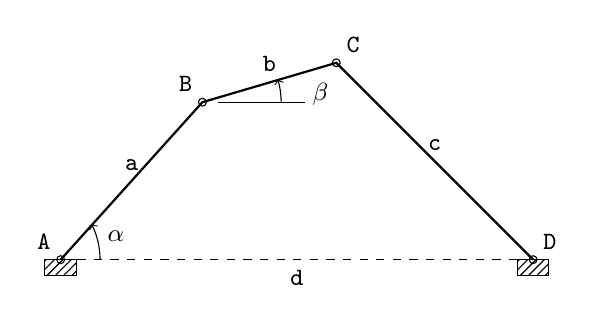
\begin{tikzpicture}[font=\small]
		\draw (0,0) node [above left] {A} circle (0.05);
		\draw (1.8,2) node [above left] {B} circle (0.05);
		\draw (3.5,2.5)node [above right] {C} circle (0.05);
		\draw (6,0) node [above right] {D} circle (0.05);
		\draw [dashed] (0,0) -- node [midway, below] {d} (6,0);
		\draw [thick] (0,0) -- node [midway, above] {a} +(1.8,2) -- node [midway, above] {b}(3.5,2.5) -- node [midway, above] {c} (6,0);
		\draw [pattern= north east lines](-0.2,-0.2) rectangle (0.2,0);
		\draw [pattern= north east lines](5.8,-0.2) rectangle (6.2,0);
		\draw [->](0.5,0) arc (0:27:1cm);
		\draw (0.7,0.3) node {$\alpha$};
		\draw (2,2) -- (3.1,2);
		\draw [->](2.8,2) arc (0:17:1cm);
		\draw (3.3,2.1) node {$\beta$};
\end{tikzpicture}
\end{document}